\documentclass{article}
\usepackage[utf8]{inputenc}
\usepackage[T1]{fontenc}
\usepackage[ngerman]{babel}
\usepackage[margin=1in,
includefoot]{geometry}%f?r rand des Textes/dokumentes
\usepackage{lipsum}%fillertext latin nonsense
\usepackage[margin=1in,left=1.5in,includefoot]{geometry}%f?r rand des Textes/dokumentes
\usepackage[hidelinks]{hyperref} % Allows for clickable references Tables preamble
\usepackage[none]{hyphenat} % Stops breaking up words in a table
\usepackage[english]{babel}
\usepackage{float} % Allows for control of float positions.
\usepackage{listings}
\usepackage{color}
%%%%%%%%%%%%%%%%%%%%%%%%%%%%%%%%%%%%%%%%%%%%%%%%%%%%%%%%%%%%%%%%%%%%%%%%%%%%%%%%
%f?r codeblocks
\lstdefinestyle{mystyle}{
    backgroundcolor=\color{backcolour},
    commentstyle=\color{codegreen},
    keywordstyle=\color{magenta},
    numberstyle=\tiny\color{codegray},
    stringstyle=\color{codepurple},
    basicstyle=\footnotesize,
    breakatwhitespace=false,
    breaklines=true,
    captionpos=b,
    keepspaces=true,
    numbers=left,
    numbersep=5pt,
    showspaces=false,
    showstringspaces=false,
    showtabs=false,
    tabsize=
}
\definecolor{codegreen}{rgb}{0,0.6,0}
\definecolor{codegray}{rgb}{0.5,0.5,0.5}
\definecolor{codepurple}{rgb}{0.58,0,0.82}
\definecolor{backcolour}{rgb}{0.95,0.95,0.92}
\lstset{style=mystyle}
%%%%%%%%%%%%%%%%%%%%%%%%%%%%%%%%%%%%%%%%%%%%%%%%%%%%%%%%%%%%%%%%%%%%%%%%%%%%%%%%
\usepackage{multicol}
\usepackage{rotating}
\usepackage{setspace}
\usepackage{lscape}
\usepackage{pdflscape}
\usepackage{float}

%shortcut for fettew?rter machen geht auch mit bfseries, wenn man das hier hat,
%muss man nur \rowstyle $ ^ ^ ^ ^  diese package ist gar nicht n?tig bei 2 table
\usepackage{array}
% \newcolumntype{$}{{\global\let\currentrowstyle\relax}}
\newcolumntype{^}{>{\currentrowstyle}}
\newcommand{\rowstyle}[1]{\gdef\currentrowstyle{#1} #1\ignorespaces}
%%%%%%%%%%%%%%%%%%%%%%%%%%%%%%%%%%%%%%%%%%%%%%%%%%%%%%%%%%%%%%%%%%%%%%%%%%%%%%%%
% Graphics preamble Allows you to import images
\usepackage{graphicx}
\usepackage[export]{adjustbox}
\usepackage{caption}
\usepackage{subcaption}
%%%%%%%%%%%%%%%%%%%%%%%%%%%%%%%%%%%%%%%%%%%%%%%%%%%%%%%%%%%%%%%%%%%%%%%%%%%%%%%%
\usepackage{float} % Allows for control of float positions.
%%%%%%%%%%%%%%%%%%%%%%%%%%%%%%%%%%%%%%%%%%%%%%%%%%%%%%%%%%%%%%%%%%%%%%%%%%%%%%%%
% Math preamble Allows us to write chemistry equations!
\usepackage{mhchem}
%f?r mathe 1/2 z.b wird richtig gezeigt.==> \sfrac{1}{2} ohne \frac{1}{2}
\usepackage{xfrac}
%%%%%%%%%%%%%%%%%%%%%%%%%%%%%%%%%%%%%%%%%%%%%%%%%%%%%%%%%%%%%%%%%%%%%%%%%%%%%%%%
% Bibliography preamble f?r Referenzen hier mit bibtex reihenfolge hyperlinking zu refer.
\usepackage[numbers,sort&compress]{natbib}
%%%%%%%%%%%%%%%%%%%%%%%%%%%%%%%%%%%%%%%%%%%%%%%%%%%%%%%%%%%%%%%%%%%%%%%%%%%%%%%%
% Bullet preamble for \begin{itemize} \item a f?r subbullet nochmals beginn und item
\renewcommand{\labelitemi}{$\bullet$}
\renewcommand{\labelitemii}{$\diamond$}
\renewcommand{\labelitemiii}{$\circ$}
%%%%%%%%%%%%%%%%%%%%%%%%%%%%%%%%%%%%%%%%%%%%%%%%%%%%%%%%%%%%%%%%%%%%%%%%%%%%%%%%
% f?r kopf und fusszeile }%macht f?r Kopf/Fusszeile strich+ man kann da dann schreiben
\usepackage{fancyhdr}
\pagestyle{fancy}
\fancyhead{}
\fancyfoot{}
\fancyfoot[R]{ \thepage\ }
\renewcommand{\headrulewidth}{0pt}
\renewcommand{\footrulewidth}{0pt}
%%%%%%%%%%%%%%%%%%%%%%%%%%%%%%%%%%%%%%%%%%%%%%%%%%%%%%%%%%%%%%%%%%%%%%%%%%%%%%%%




















\begin{document}
\begin{titlepage}
    \begin{center}
    \line(1,0){500} \\ %macht eine linie mit durchmesser 300
    [3mm]%h?he der Linie
    \huge{\bfseries Meine Flask-Webseite mit mini-Game} \\
    [2mm]%h?he der Linie
    \line(1,0){300} \\ %macht eine linie mit durchmesser 200
    [1.5cm]%abstand h?he
    \textsc{\LARGE IDPA} \\
    [0.75cm]
    \text{Bitte schau dir mein Code auf Github/alcatraz5yz an} \\
    \text{}{ Und sieh dir meine hochgeladene Webseite auf idpa.herokuapp.com an}\\








\vspace{2cm}
    \begin{figure}[ht]
    \centering
    \begin{subfigure}{.5\textwidth}
      \centering
      
\includegraphics[width=.5\linewidth]{git_logo}
      \caption{Version control}
      \label{fig:sub1}
    \end{subfigure}%
    \begin{subfigure}{.5\textwidth}
      \centering
      
\includegraphics[width=.5\linewidth]{phaser}
      \caption{phaser}
      \label{fig:sub2}
    \end{subfigure}
    % \caption{}
    % \label{fig:test}
    % \caption[short title]{}
    \end{figure}
    \vspace{3cm}












    \end{center}
    \begin{flushright}
    \textsc{
    \large Schueler: Allan Kueng\\
    Abgabedatum: 19 Mai 2017 \\
    Lehrperson: Herr Ragazi\\
    }
    \end{flushright}
\end{titlepage}


% Front matter stuff
\pagenumbering{roman}


% This is table of contents stuff
\renewcommand{\contentsname}{Inhaltsverzeichnis}
\tableofcontents
\thispagestyle{}%keine Seitenzahl mehr
\renewcommand{\footrulewidth}{3pt}
\fancyfoot[c]{Projektarbeit}
\cleardoublepage




% List of pictures
\listoffigures
\addcontentsline{toc}{section}{\numberline{}List of Figures}
\cleardoublepage


%list of tables
% \listoftables
% \addcontentsline{toc}{section}{\numberline{}List of Tables}
% \cleardoublepage

\section*{Zielsetzung}
% \addcontentsline{toc}{section}{\numberline{}Summary}%f?gt summary mit i zu table of contents
Mein Ziel ist es eine Funktionst?chtige Webseite mit Login/ Gallery/Blog/und Game zu erstellen und dies noch auf einen Cloud Dienst Hochzuladen.
Da ich erst vor einem halben Jahr angefangen habe programmieren zu lernen und f?r dieses Projekt f?nf Programmiersprachen brauche,
Werde ich sicher noch in Stress kommen, das heisst ich muss zuerst noch die Sprachen lernen.
Das Dokument will ich nicht wie alle anderen mit Word schreiben sondern auch mit einer Programmiersprache n?mlich Latex.
\cleardoublepage



% This is main body stuff nach einf?hrung, hauptteil
\pagenumbering{arabic}
\setcounter{page}{1}%nach thispagestyle wieder mit seitenzahl 1 anfangen
%%%%%%%%%%%%%%%%%%%%%%%%%%%%%%%%%%%%%%%%%%%%%%%%%%%%%%%%%%%%%%%%%%%%%%%%%%





\section{Zeitplan}

\begin{sidewaysfigure}[h!]
  % \renewcommand{\textfraction}{0.005}
    \centering
    % \noindent\includegraphics[width=\linewidth,height=.<7\textheight,keepaspectratio]{/}
    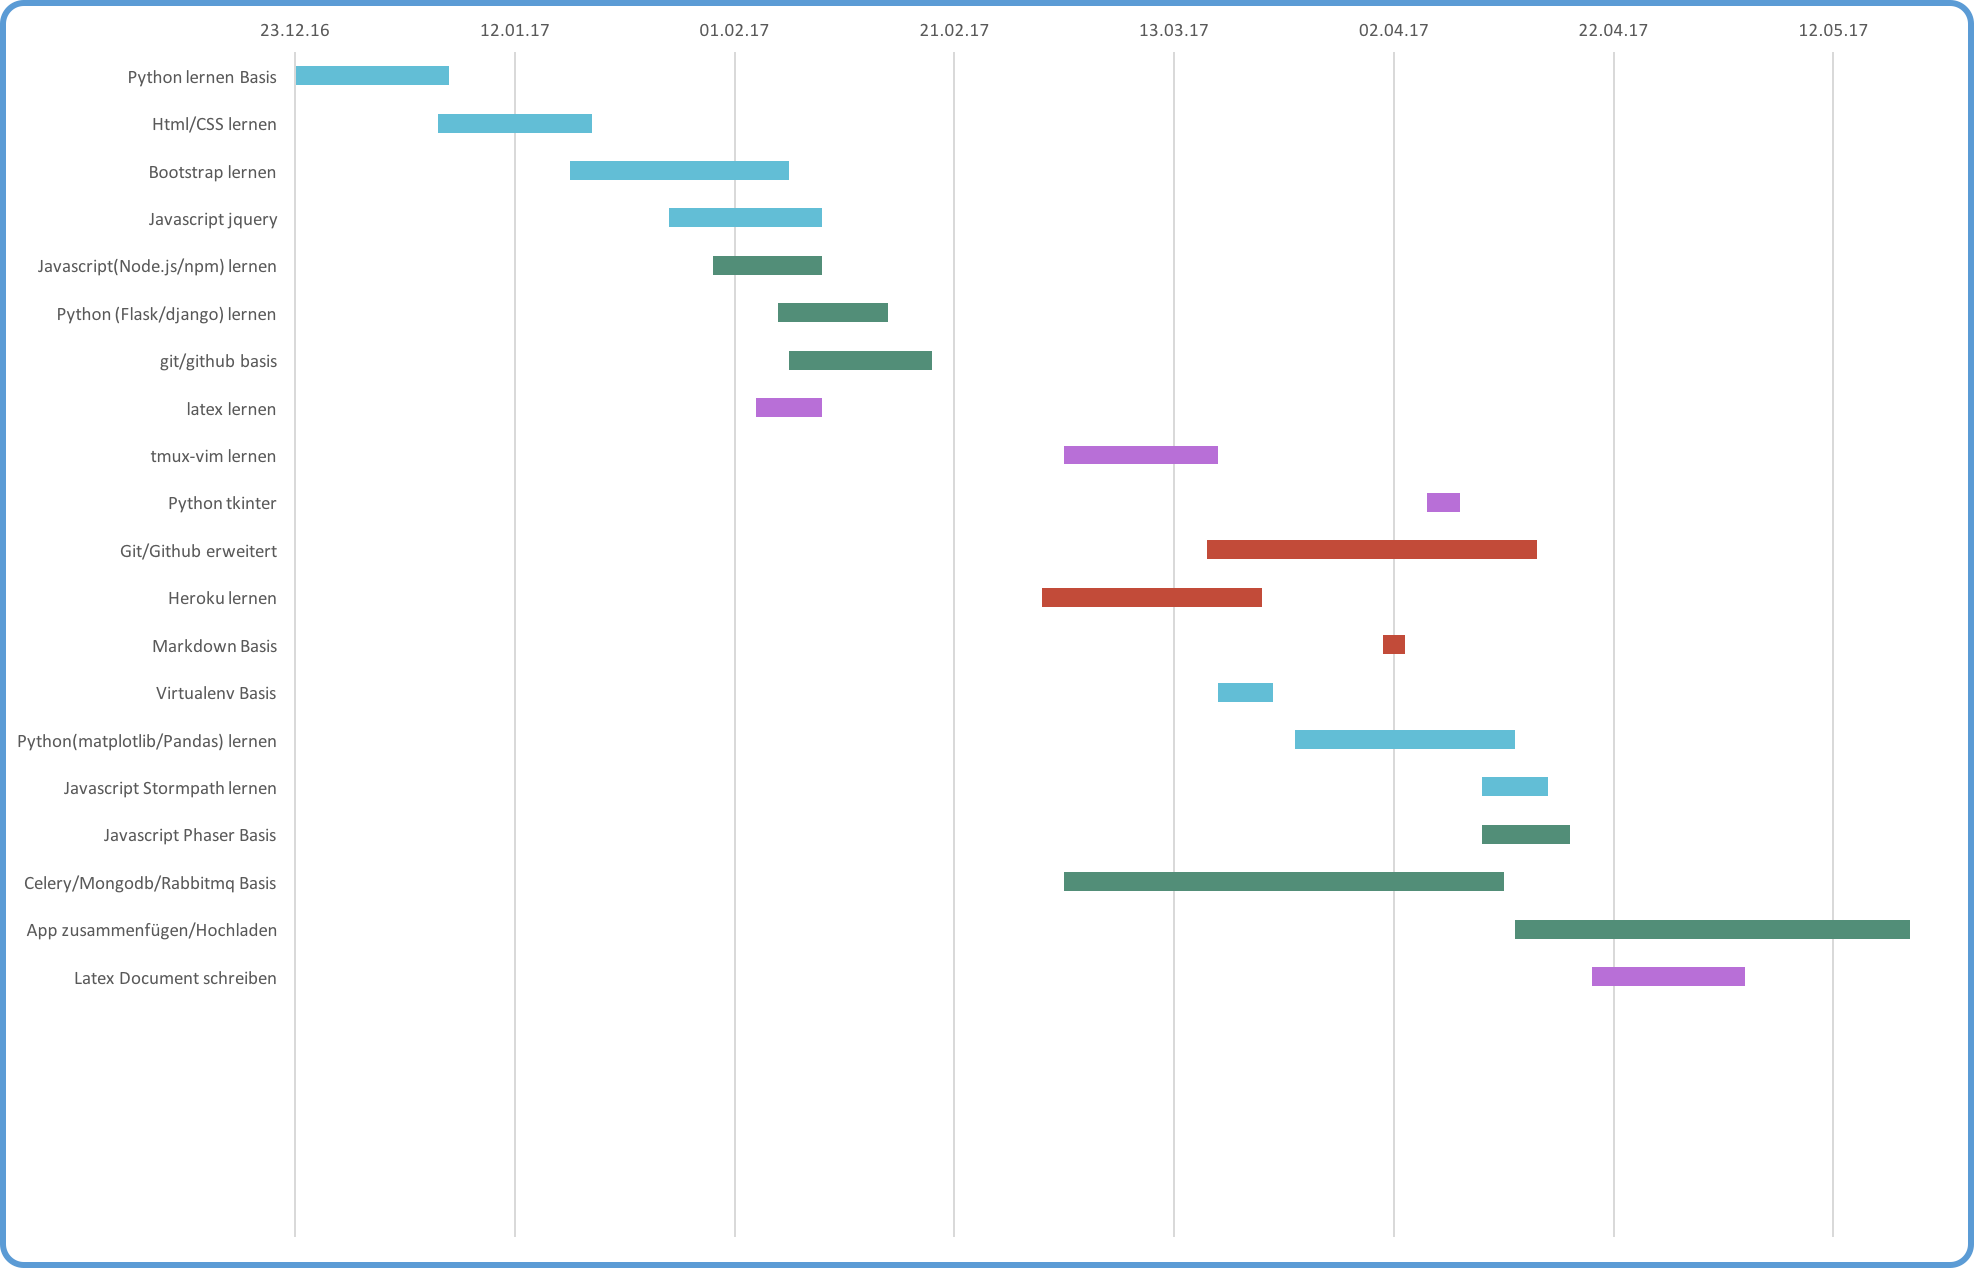
\includegraphics[width=.8\linewidth]{gantt}
    \caption{Version control}
    \label{fig:sub1}
    \end{sidewaysfigure}





\cleardoublepage


\section{Allgemeines}
In Dieser Arbeit befinden sich im Haupteil drei Einzelne Kapitel.
das Erste wird ?ber die Grundlagen des Programmierens sein, wo ich zeigen werde wie und mit welchen Mitteln ich meine Webseite erstellt habe.
im Zweiten teil wird es um den Aufbau und die Struktur meiner Webseite gehen und im dritten Teil geht es um das Minigame,
welches ich mit der Engine Phaser erstellt habe.

Ich will noch betonen dass diese Arbeit sehr komplex ist und ich nat?rlich nicht in der Lage sein werde dir alles genau zu erkl?ren, da diese Arbeit ja
um die 40 Seiten umfasst. Falls du dich aber nach dem Lesen auch daf?r interessieren solltest selber etwas zu erstellen, habe ich im Anhang noch einige Quellen
aufgelistet, welche dir helfen sollten selber durchzustarten.


\begin{figure}[ht]
    \centering
    
\includegraphics[width=.7\linewidth]{foto}
    \caption{Startbild meines Games}
    \label{fig:sub1}
    \end{figure}

\cleardoublepage












\section{html}
Hypertext Markup Language oder kurz HTML ist die Grundsprache wenn es darum geht eine Webseite zu Programmieren.
 Sie ist eine textbasierte Auszeichnungssprache zur Strukturierung digitaler Dokumente wie Texte mit Hyperlinks, Bildern und anderen Inhalten.
 HTML-Dokumente sind die Grundlage des World Wide Web und werden von Webbrowsern dargestellt.
 Neben den vom Browser angezeigten Inhalten k?nnen HTML-Dateien zus?tzliche Angaben in Form von Metainformationen enthalten, z. B.
?ber die im Text verwendeten Sprachen, den Autor oder den zusammengefassten Inhalt des Textes.
Kurz gesagt erstellt man damit die Grundstruktur der Webseite.
Oder wenn man sich die Webseite als Haus vorstellt ist HTML die W?nde und Dach/Boden.
Ein HTML document hat immer die Endung .html und man kann es direkt im Browser aufrufen ohne es vorher noch Kompilieren zu m?ssen, was sehr n?tzlich ist.
Zum Inhalt:
Ein html file besteht immer aus Head und Body und wird wie alles andere auch in Form von Tags geschrieben.
ein Beispiel <head></head> ist der head, zwischen <head> und </head> kommt der ganze Rest hinein.

Hier ein kleines Allgemeines Beispiel(Ich zeige ein allgemeines Beispiel, weil code aus meiner Website etwas komplizierter ist als "normaler html-code")

\begin{figure}[ht]
    \centering
    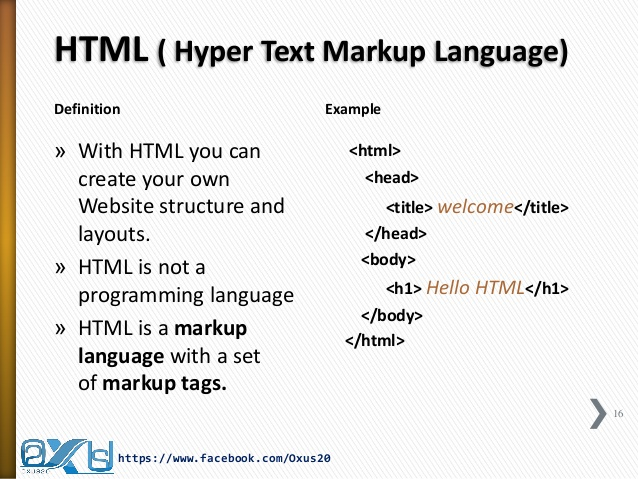
\includegraphics[width=.7\linewidth]{html-wissen}
    \caption{html-aufbau}
    \label{fig:sub1}
    \end{figure}
Zus?tzlich muss man ganz oben im head auf alle css files hinweisen, welche das html-dokument braucht z.B.:

\begin{lstlisting}
<link rel="stylesheet" href="/static/css/main.css"
\end{lstlisting}

Das gleiche f?r javascript-files, einfach im body ganz unten. z.B.:

\begin{lstlisting}
<script src="phaser.min.js"
\end{lstlisting}








\cleardoublepage


\section{css}
Cascading Style Sheets oder kurz css geh?rt wie HTMl zur Grundstruktur wenn man eine Webseite gestalten will.
Diese Sprache ist vergleichbar mit Farbe, denn mit ihr will man die Seite sch?ner und attraktiver Gestalten.
css ist ein "living standard", das heisst sie wird st?ndig weiterentwickelt.
Bei css benutzt man nicht wie bei html tags wie <head></head> sondern es sieht in etwa so aus:\\
\begin{lstlisting}
  body {
    font-size: 1em;
    color: #777B7E;
    font-weight: 400;
    background: #D3D8DC;
    position: relative;
  }
\end{lstlisting}







Mit css arbeitet man so:\\
man w?hlt den Oberbegriff aus dem Html-File (hier body)\\
dann setzt man in Klammern ({}) was ver?ndert werden soll.\\
man kann w?hlen zwischen vielen Sachen wie z.B. der H?he oder der Breite.\\
Nat?rlich muss man im html-File angeben, dass man dieses css-File benutzt um
ver?nderungen and der Struktur der Seite vorzunehmen.\\
Diese Referenz sieht dann wie folgt aus:


\begin{lstlisting}
<link rel="stylesheet" href="/static/css/main.css"
\end{lstlisting}


\begin{figure}[ht]
    \centering
    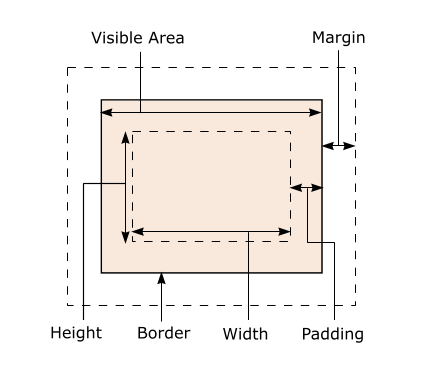
\includegraphics[width=.7\linewidth]{css-box}
    \caption{css aufbau}
    \label{fig:sub1}
    \end{figure}

\cleardoublepage


\section{jquery}






Jquery ist ein Framework welches auf Javascript basiert.
Jquery wird benutzt um animationen und andere Funktionen in die Webseite hineinzubringen.
Ich benutze einige Jquery-Plugins welche ich von der Webseite jqueryrain herhabe.
Von dieser Seite hole ich mir die Komplexen Codebl?cke, welche ich noch in mein eigenes Framework einf?gen muss.
ich muss sie noch ver?ndern damit sie genau in meine Webseite hineinpasst.









\section{meine jquery-Plugins}

\begin{figure}[ht]
    \centering
    
\includegraphics[width=.6\linewidth]{sticky}
    \caption{Das Sticky-Plugin erlaubt es mir beim Herunterscrollen gewisse Textstellen festzuhalten.}
    \label{fig:sub1}
    \end{figure}

    \begin{figure}[ht]
        \centering
        
\includegraphics[width=.6\linewidth]{carousel}
        \caption{Javascript und jquery logo}
        \label{fig:sub1}
        \end{figure}

        \begin{figure}[ht]
            \centering
            
\includegraphics[width=.6\linewidth]{gallery}
            \caption{Javascript und jquery logo}
            \label{fig:sub1}
            \end{figure}

            % \begin{figure}[ht]
            %     \centering
            %     
\includegraphics[width=.5\linewidth]{paint}
            %     \caption{Javascript und jquery logo}
            %     \label{fig:sub1}
            %     \end{figure}
            %
            %     \begin{figure}[ht]
            %         \centering
            %         
\includegraphics[width=.5\linewidth]{background}
            %         \caption{Javascript und jquery logo}
            %         \label{fig:sub1}
            %         \end{figure}
            %
            %         \begin{figure}[ht]
            %             \centering
            %             
\includegraphics[width=.7\linewidth]{modernizr}
            %             \caption{Javascript und jquery logo}
            %             \label{fig:sub1}
            %             \end{figure}








\cleardoublepage



\section{Flask}


\subsection{Python-allgemein}

Python ist eine Interpretierte, object-orientierte programmiersprache mit dynamischer Semantic.
Python is einfach zu lernen im Vergleich zu C oder Java und sie ist auch sehr einfach zu lesen.
Programmierer suchen sich auch oft diese Programmiersprache aus, weil man Fehler einfach finden kann man sich dadurch viel Wartung erspart.
Wenn du mehr ?ber Python erfahren willst, gehe doch zur Python hauptseite unter www.python.org
\subsection{flask-allgemein}

Flask ist ein in Python geschriebenes Webframework. Der Fokus von Flask liegt auf Erweiterbarkeit und guter Dokumentation.
Die einzigen Abh?ngigkeiten sind Jinja2,
eine Template Engine, und Werkzeug, eine Bibliothek zum Erstellen von WSGI-Anwendungen.
\subsection{flask-vereinfacht}
Flask ist wie der Backend Router der zeigt wo welche seite erscheint und mir viele Werkzeuge zur Verf?gung stellt.
Um Flask laufen zu lassen, muss ich nur python app.py im richtigen Ordner im Terminal eingeben, wobei app.py das File ist
% z.B: kann ich meine Flask-Webseite lokal im Browser auf Pfad 8080 laufen lassen, wenn ich im terminal eingebe
% cd idpa
% python app.py
% und sehe bei der URL-Pfad:
% dass es die Index seite geladen hat, wie ich es im Python-router-file programmiert habe.


\begin{figure}[ht]
    \centering
    
\includegraphics[width=.5\linewidth]{flask}
    \caption{Version control}
    \label{fig:sub1}
    \end{figure}

von Flask importiere ich alles n?tigen Bibliotheken um mein Project z.B:\\
Sicherer zu machen beim Login. Dies mithilfe von der Bibliothek:
\begin{lstlisting}
from flask_bcrypt import generate_password_hash
\end{lstlisting}
welches ich im File models.py eingef?gt habe.
Dies erlaubt es mir



\cleardoublepage

\section{Datenbanken}
Die Programmiersprache mit welcher man Datenbanken programmieren kann heisst. sql oder sequel:
Datenbanken werden gebraucht um Daten darin zu speichern, es gibt viele verschiedene Arten, ich habe mich f?r sqlite entschieden, weil sie eher eine einfache version ist und vor allem f?r Anf?nger gedacht ist.
Ich habe also die Datenbank genannt sqlite mithilfe der Pythonbibliothek genannt Peewee erstellt.
Dank Peewee musste ich nicht auch noch die Programmiersprache sql lernen, bei der es um Datenbanken geht, denn Peewee erstellt mir einfach eine.



\begin{figure}[ht]
    \centering
    
\includegraphics[width=.5\linewidth]{database}
    \caption{Logo Databases}
    \label{fig:sub1}{Wie sie sehen gibt es verschiedene Arten von Datenbanken.}
    \end{figure}

    \begin{figure}[ht]
        \centering
        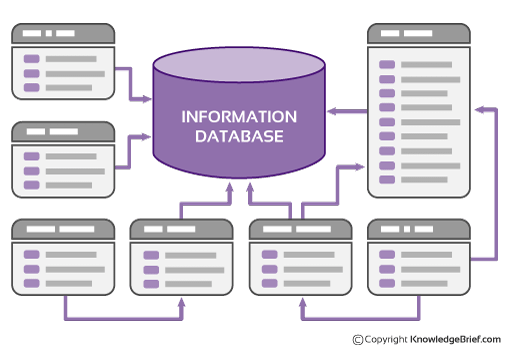
\includegraphics[width=.8\linewidth]{database1}
        \caption{Logo Databases}
        \label{fig:sub1}{Wie sie sehen gibt es verschiedene Arten von Datenbanken.}
        \end{figure}
% Nun zu meinem project:\\
% in meinem Project habe ich ein File welches models.py heisst, darin steht:
%
%
%
%     \begin{lstlisting}
%       from peewee import *
%       DATABASE = SqliteDatabase('social.db')
%     \end{lstlisting}
%     Hier f?ge ich die Datenbank sqlite mithilfe von peewee ein.\\
%
%   weiter unten im selben File kann man sehen:
%     \begin{lstlisting}
%     def initialize():
%     DATABASE.connect()
%     DATABASE.create_tables([User, Post, Relationship], safe=True)
%     DATABASE.close()
%     \end{lstlisting}
%

\cleardoublepage































\section{Text Editor}

Programmieren tut man nicht mit Word oder Excel oder Powerpoint.
Man braucht einen anst?ndigen Text Editor,
welcher mit wichtigen Sachen wie zum Beispiel syntax highlighting ausgestattet ist, damit man seinen Code besser betrachten kann.
Zudem kann ein Text Editor vieles was man eigentlich im Terminal tun m?sste, und kann es sogar leichter und schneller machen.
Jeder Anf?nger im Programmieren weiss, dass man einen Text Editor braucht gut Programmieren zu k?nnen.
Die Frage ist nur (und das besch?ftigt auch fortgeschrittene Programmierer) welcher man verwenden sollte.
Ich habe Meine Webseite im Text Editor Atom und das Game in Brackets programmiert.
Atom weil es feature-reich ist und brackets wegen der Livevorschau, welche es mir erm?glicht ver?nderungen von meinem Game Live anzusehen.
\begin{figure}[ht]
    \centering
    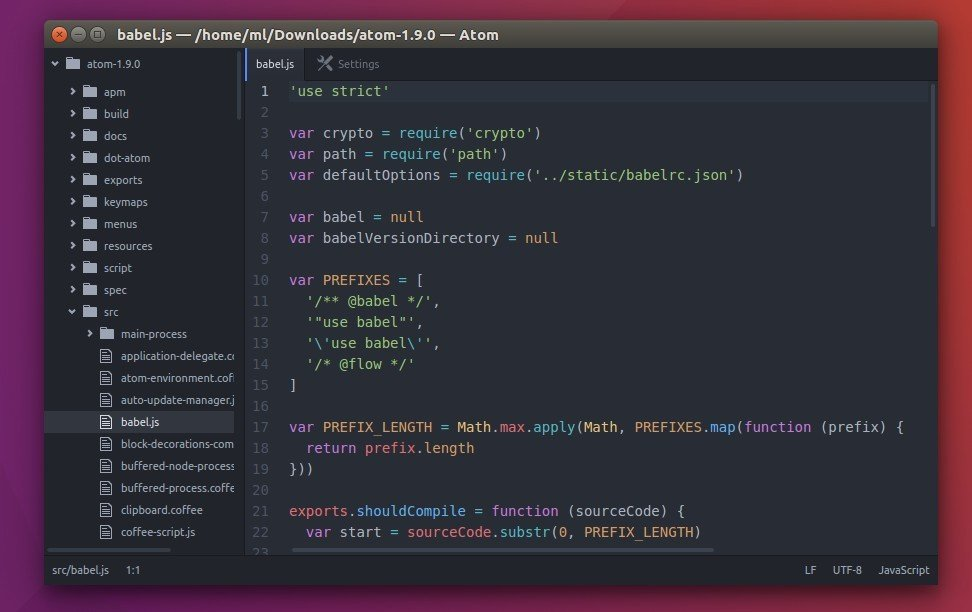
\includegraphics[width=.6\linewidth]{text-editor}
    \caption{Beispiel Terminal}
    \label{fig:sub1}{Hier sehen sie den Text Editor Atom.\\
    Links befindet sich die Auflistung aller Files und Ordner\\
    Rechts ist der Platz wo man Code schreibt}
    \end{figure}




    \begin{figure}[ht]
        \centering
        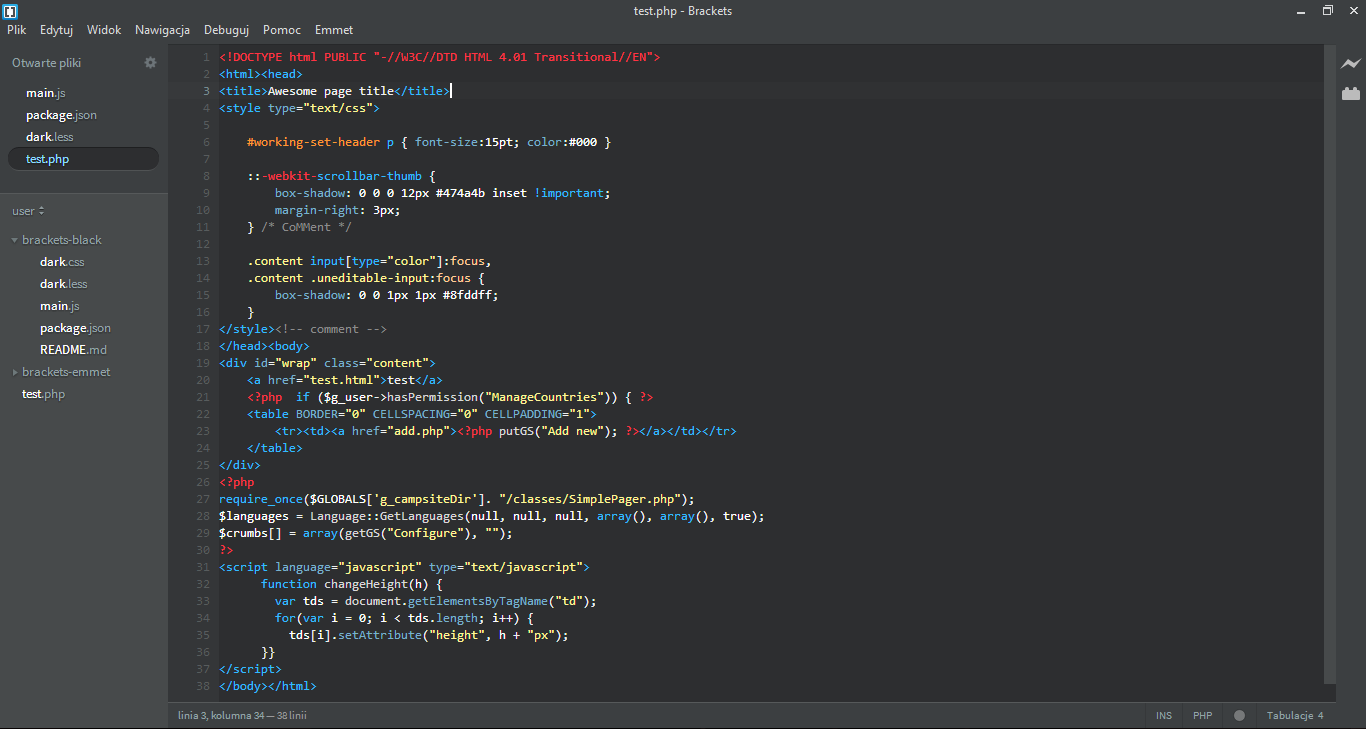
\includegraphics[width=.6\linewidth]{brackets}
        \caption{Beispiel Terminal}
        \label{fig:sub1}{Brackets ist ?hnlich wie Atom aufgebaut.\\
        Zu beachten ist rechts oben der LiveVorschau-knopf.}
        \end{figure}

\cleardoublepage












\section{Git und Github}
Git ist ein freies und open source Kontrollsystem um alles von kleinen zu gr?sseren
Projecten zu handeln.
Git ist einfach zu lernen und hat zugleich eine mega schnelle Verarbeitungsgeschwindigkeit
Es ist besser als manch andere SCM (bla bal) tools wie etwa Subversion, CVS, Perforce
und ClearCase.
Mit Features wie etwa einfaches teilen seiner arbeiten, bequemes staging und multiple Workflows.
\begin{figure}[ht]
\centering
\begin{subfigure}{.5\textwidth}
  \centering
  
\includegraphics[width=.5\linewidth]{git_logo}
  \caption{gitlogo}
  \label{fig:sub1}
\end{subfigure}%
\begin{subfigure}{.5\textwidth}
  \centering
  
\includegraphics[width=.5\linewidth]{github}
  \caption{Githublogo}
  \label{fig:sub2}
\end{subfigure}
% \caption{}
% \label{fig:test}
% \caption[short title]{}
\end{figure}

\begin{figure}[ht]
    \centering
    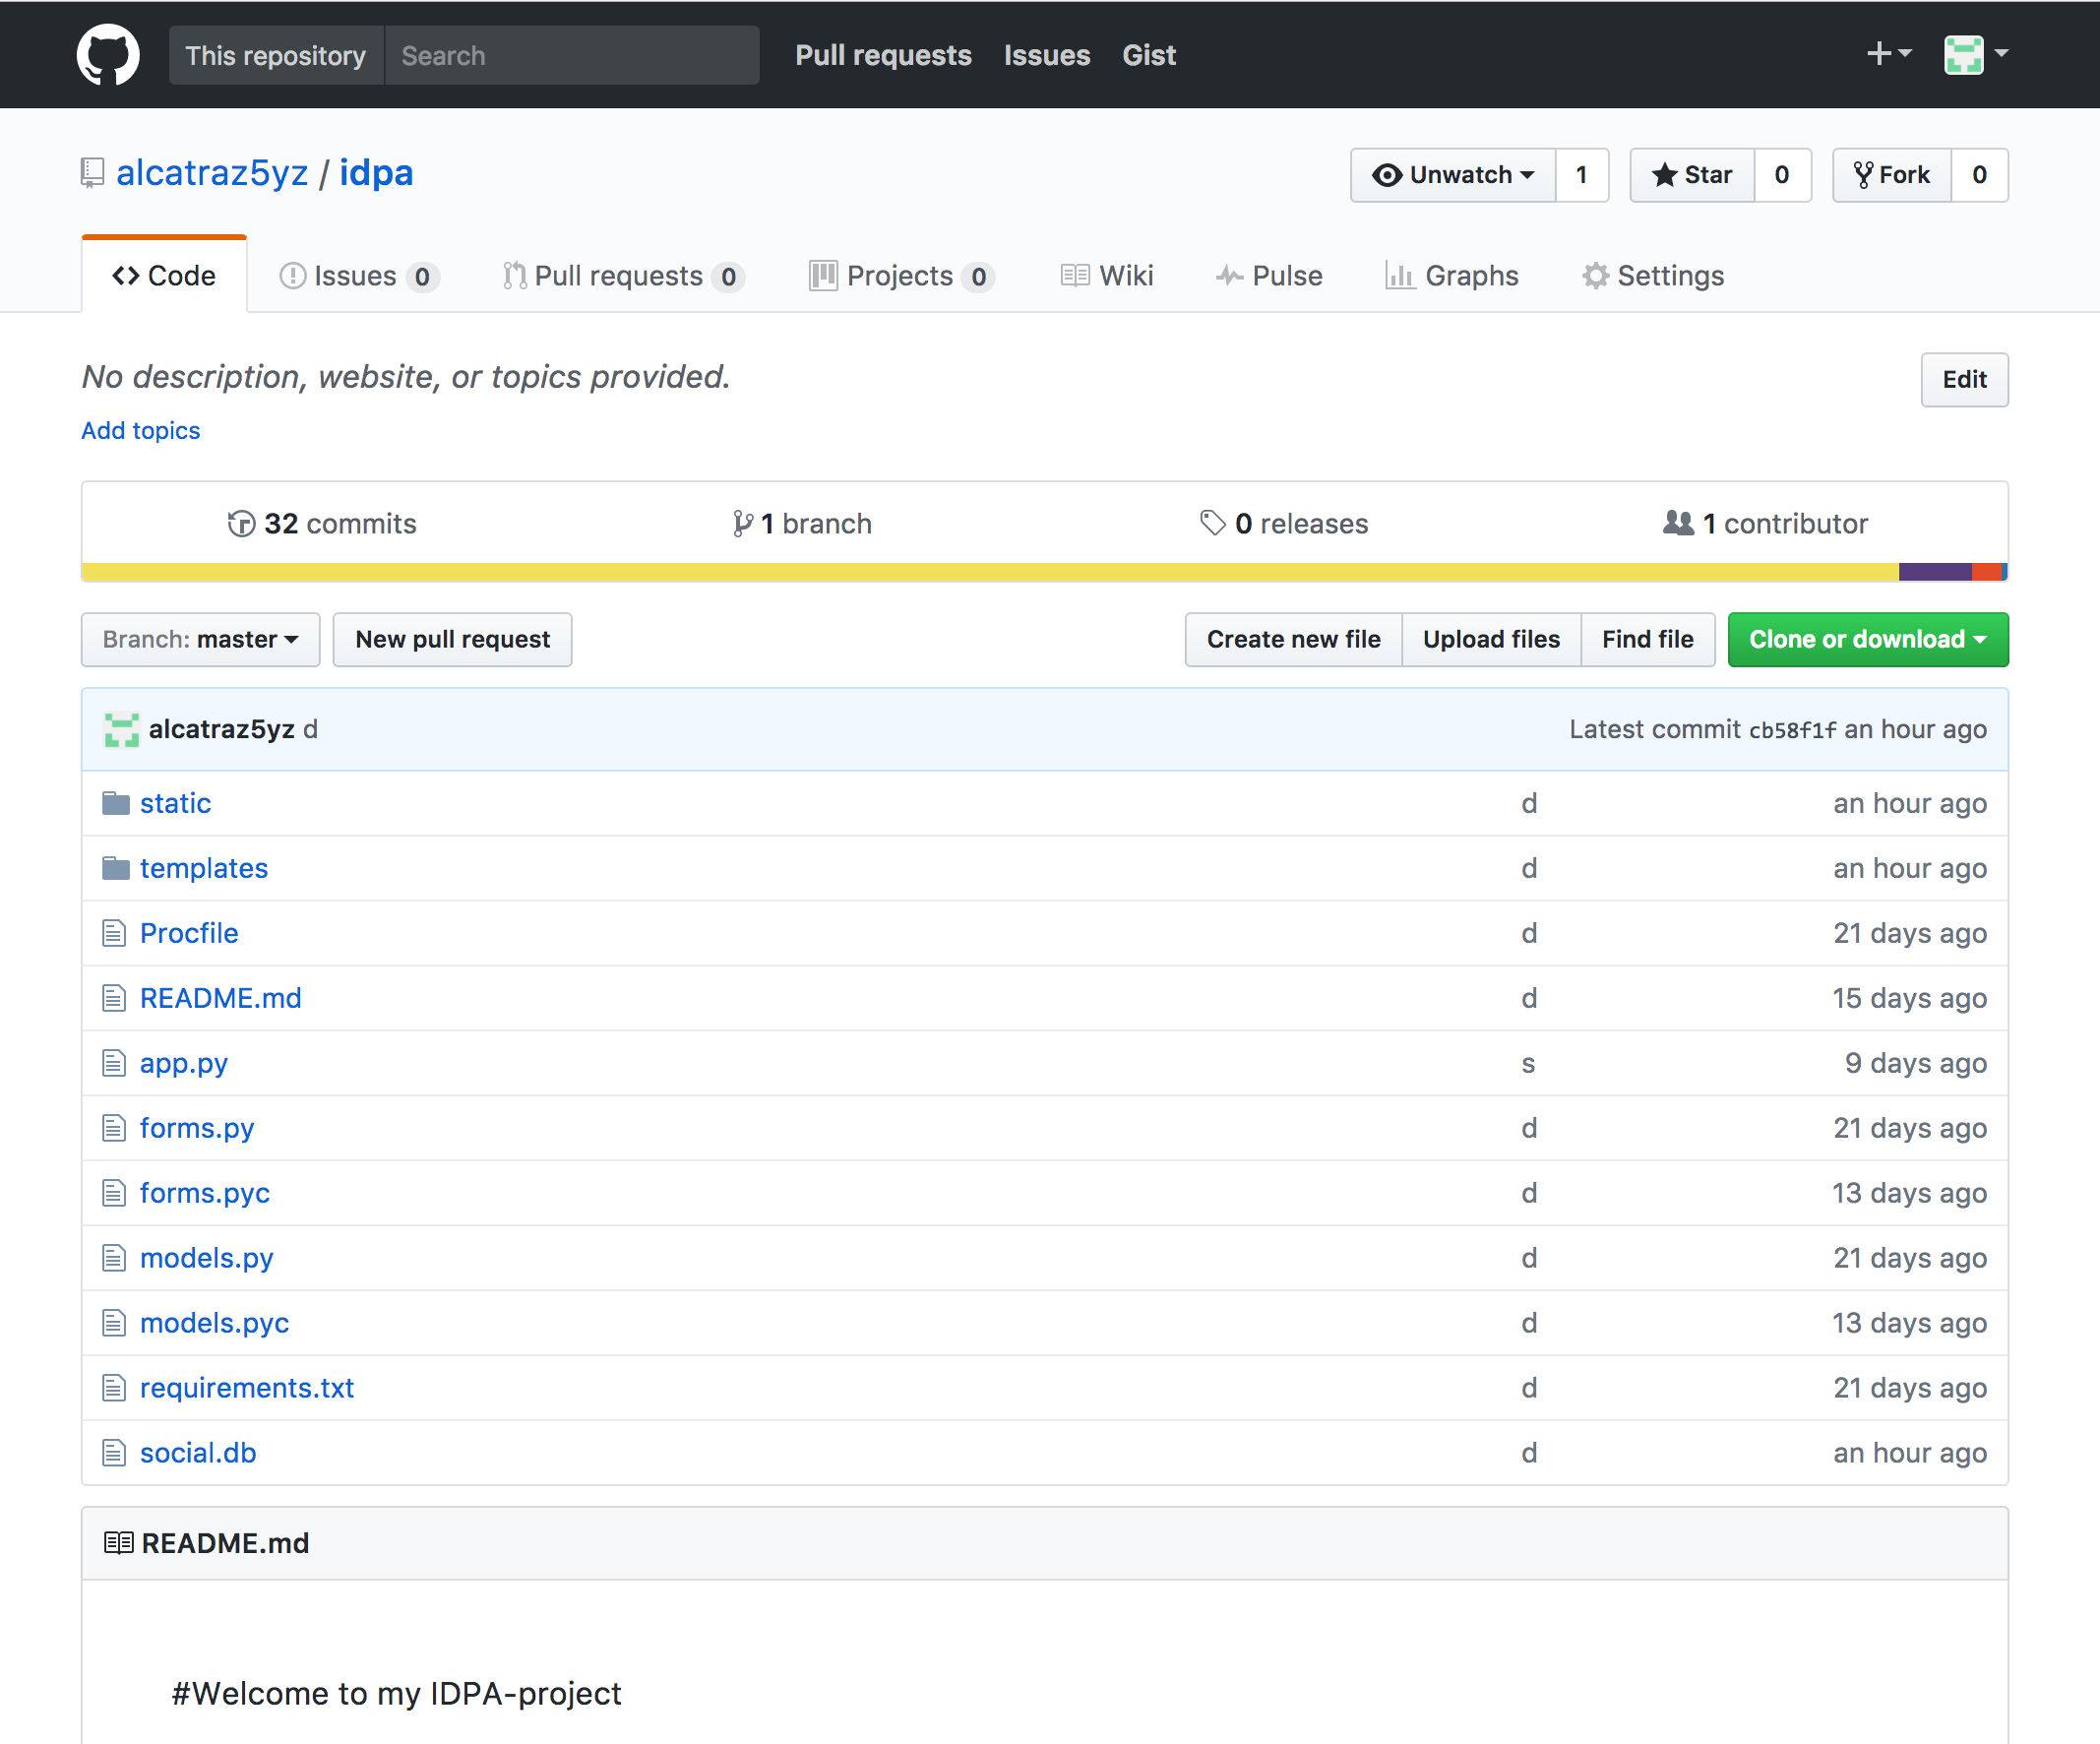
\includegraphics[width=.7\linewidth]{github-repo}
    \caption{Version control}
    \label{fig:sub1}
    \end{figure}

    % \begin{figure}[ht]
    %     \centering
    %     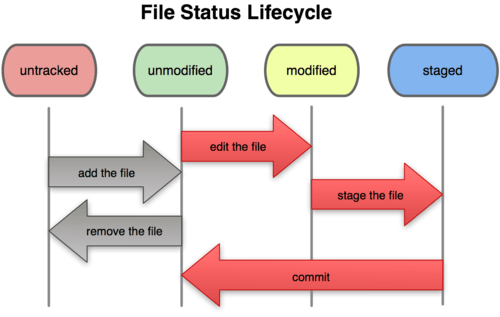
\includegraphics[width=.7\linewidth]{git}
    %     \caption{Hier sieht }
    %     \label{fig:sub1}
    %     \end{figure}

\cleardoublepage











% \section{Bower}
% Bower ist ein netter kleiner Helfer, der es mir Erm?glicht Plugins z.B. von Jquery bequem von meinem Terminal in mein Project einzubinden, ohne auf die
% jeweilige Webseite gehen zu m?ssen und den Code da zu suchen.
%
%
% \begin{figure}[ht]
%     \centering
%     
\includegraphics[width=.5\linewidth]{bower}
%     \caption{Version control}
%     \label{fig:sub1}
%     \end{figure}
%
% \cleardoublepage

\section{phaser Engine}
Phaser ist eine game-Engine welche als Basis (mit eingebauter Physik und anderer Logik) daf?r dient, sein eigenes Spiel darauf zu erstellen.
Phaser ist eine gute Gameengine welche f?r Anf?nger geeignet ist, ich zum Beispiel habe in wenigen Wochen ein eigenes Minispiel kreieren k?nnen mit
relativ kleinem Aufwand.\\
Mit eingebauter Physik meine ich das man Figuren in sein eigenes Game einbetten kann, welche and Physikalische Gesetze gebunden sind.
das heisst ich kann einen Stein in mein Game einbinden und ihn dann so programmieren, dass er z.B. immer herunterf?llt, wenn ihn der Spieler anst?sst.
\begin{figure}[ht]
\centering
\begin{subfigure}{.5\textwidth}
  \centering
  
\includegraphics[width=.5\linewidth]{phaser}
  \caption{gitlogo}
  \label{fig:sub1}
\end{subfigure}%
\begin{subfigure}{.5\textwidth}
  \centering
  
\includegraphics[width=.5\linewidth]{foto}
  \caption{Githublogo}
  \label{fig:sub2}
\end{subfigure}
% \caption{}
% \label{fig:test}
% \caption[short title]{}
\end{figure}

\cleardoublepage














\section{Latex}
Latex ist eine Programmiersprache, welche es mir erm?glicht dokumente wie mit Word zu schreiben.
Mit Latex muss man die Einstellungen selber Programmieren, was man mit Word nicht muss.
Bei Word ist das so, dass man zwar nicht selber programmieren muss, daf?r muss man aber den richtigen Abschnitt mit dem Richtigen Knopf finden.
Wenn man also ein schneller Typer ist und die Befehle auswendig kann, ist man viel schneller mit Latex als mit Word, weil man nicht erst noch die Kn?pfe suchen muss.
Zus?tzlich kann man mit Latex Mathematische Formeln viel einfacher auflisten und darstellen.
Da man mit Latex alles selber programmieren muss, kann man auch genau sagen wo welcher Text hin soll.
Dad heisst kein h?ssliches Verschieben des Textes mehr wie in Word.

Aufbau: Das Latex-File ist wie ein html-File aufgebaut, das heisst es besteht aus "head" welcher die Pakete beinhaltet welche man braucht und aus "body"
welcher die Oberfl?che darstellt, welche man ansehen kann.
Falls du es nocht nicht gemerkt hast, dieses Dokument wurde ebenfalls mit Latex erstellt.


\begin{figure}[ht]
    \centering
    
\includegraphics[width=.6\linewidth]{latex-plakat}
    \caption{Version control}
    \label{fig:sub1}
    \end{figure}

\cleardoublepage
















\section{heroku}
Heroku ist ein Cloud dienst welcher es mir erm?glicht meine Flask-Webseite hochzuladen.
Heroku ist auf einige Sprachen und Frameworks besonders gut ausger?stet, welches es erleichtert sie Hochzuladen falls es irgendwelche ausnahmen gibt.
Heroku ist gratis bis zu einem bestimmten Punkt, das heisst man kann bis zu 5 Webseiten gratis hochladen.
die Downsite ist, dass die hochgeladene Seite die URL z.B. www.Beispiel.herokuapp.com hat. (Siehe herokuapp ist darin enthalten.)

F?r Programmierer ist es sehr bequem ihre Seite auf Heroku zu laden, denn man kann sie einfach in dem Terminal hochladen und muss nicht extra auf die Seite
von Heroku gehen und sie dort hochladen, es geht aber nat?rlich auch.


\begin{figure}[ht]
    \centering
    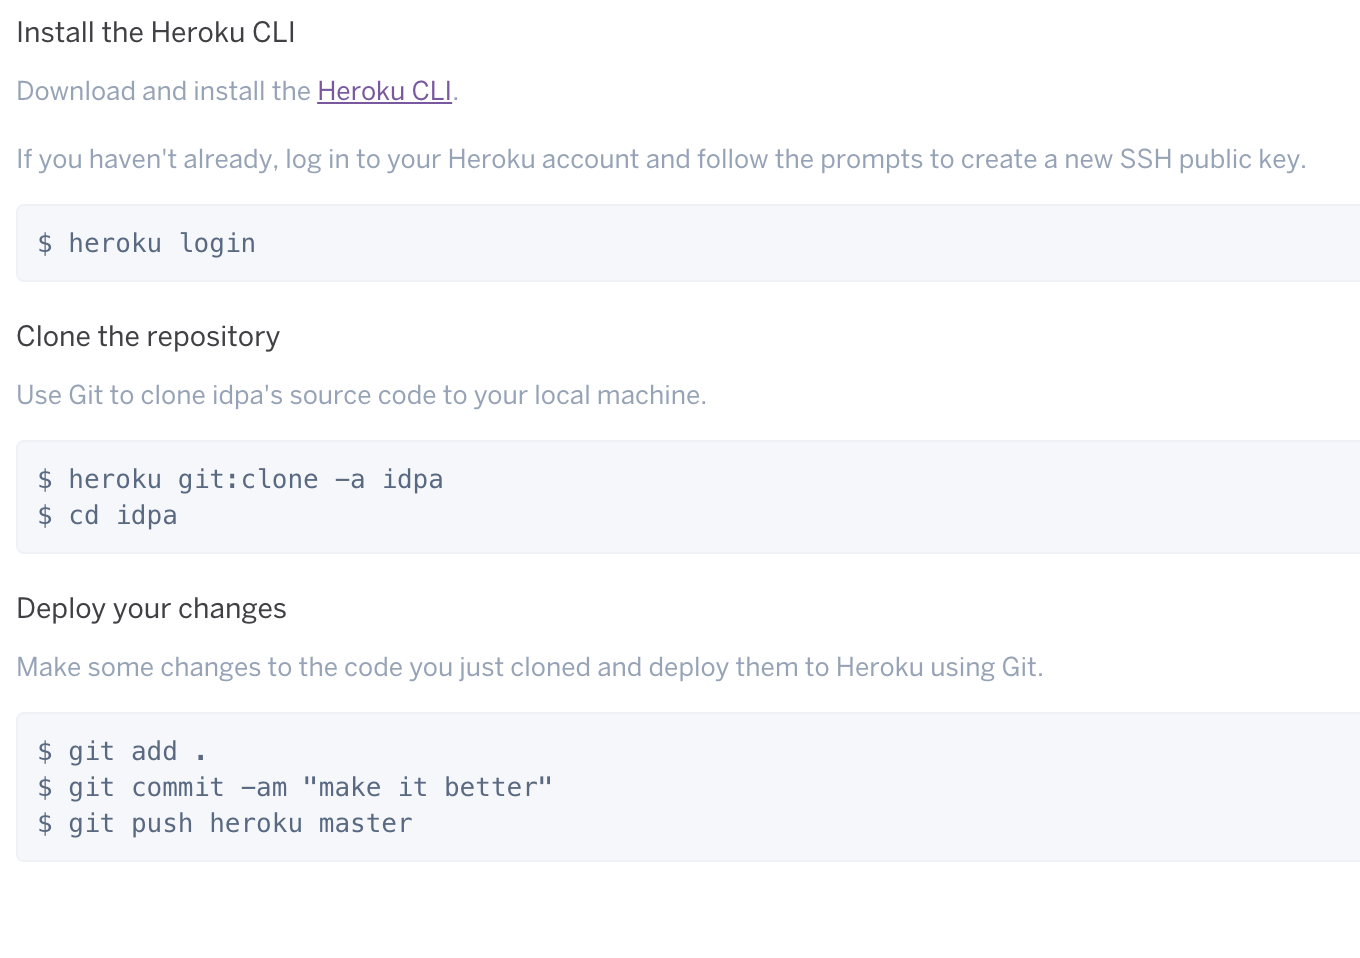
\includegraphics[width=.6\linewidth]{heroku-instructions}
    \caption{Dies ist ein Bild von der Heroku webseite:\\
    man sieht es hat dort eine gute erkl?rung wie man alles Handeln kann.}
    \label{fig:sub1}
    \end{figure}

    \begin{figure}[ht]
        \centering
        
\includegraphics[width=.7\linewidth]{heroku-pipeline}
        \caption{Es gibt auch zus?tzliche Features}
        \label{fig:sub1}
        \end{figure}




\begin{figure}[ht]
    \centering
    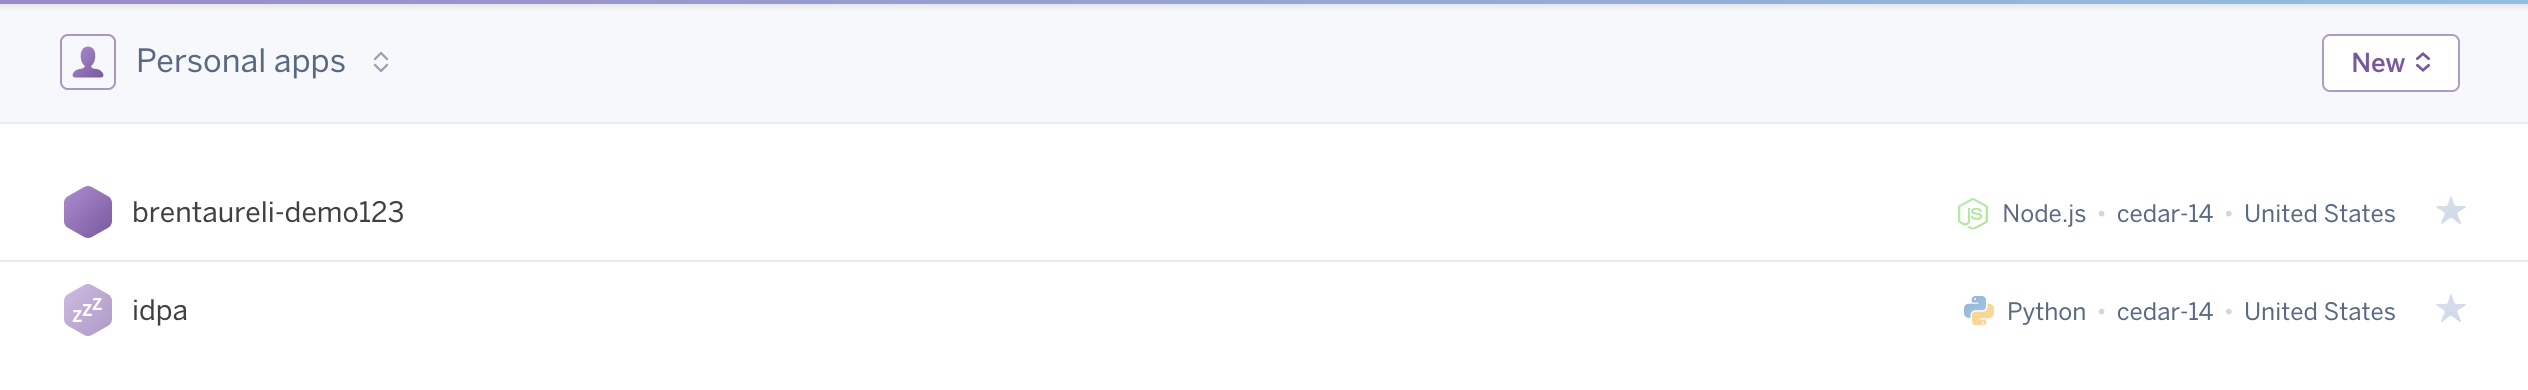
\includegraphics[width=.8\linewidth]{heroku-apps}
    \caption{Hier sieht man meine Apps welche ich auf Heroku hochgeladen habe, das einte ist meine idpa}
    \label{fig:sub1}
    \end{figure}
\cleardoublepage






\section{CLI/Terminal/cmd/Powershell/iTerm}


\begin{figure}[ht]
\centering
\begin{subfigure}{.5\textwidth}
  \centering
  
\includegraphics[width=.5\linewidth]{download-1}
  \caption{logo cmd}
  \label{fig:sub1}
\end{subfigure}%
\begin{subfigure}{.5\textwidth}
  \centering
  
\includegraphics[width=.5\linewidth]{download-2}
  \caption{allgemeines Logo}
  \label{fig:sub2}
\end{subfigure}
% \caption{}
% \label{fig:test}
% \caption[short title]{}
\end{figure}


Eines der vermutlich wichtigsten Tools ist wohl der Terminal unter Windows Usern auch als CMD bekannt.
Mit dem Terminal kann man so ziemlich alles machen.\\
man kann sogar zwei arten von Text Editoren im Terminal laufen lassen(vim und nano).
Ich mache meine Arbeit aber mit Atom und Brackets.\\
\subsection{Wof"ur ich den Terminal alles brauche}

Ich benutze den Terminal f"ur vielerlei:\\
1. um Meine erstellte Webseite Lokal laufen zu lassen und zu schauen ob sie geht\\
2. um meinen Code auf Github zu laden und zu holen wenn n?tig,das heisst mein Code verwalten.\\
3. um meinen Code auf Heroku zu laden\\
4. um allgemeines zeugs zu tun wie etwa neues file/Ordner erstellen\\
5.
6.\\



\begin{figure}[ht]
    \centering
    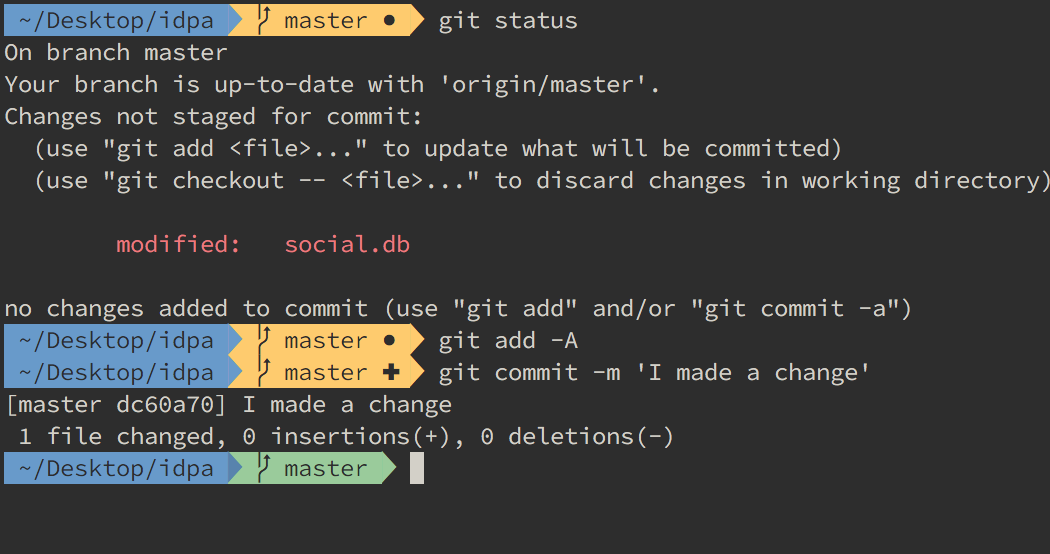
\includegraphics[width=.7\linewidth]{cli}
    \caption{Beispiel Terminal}
    \label{fig:sub1}{Hier sehen sie mein Terminal,(
    ich benutze iTerm auf meinem Macbook Pro),
    worin ich gerade
    die Version von meinem Project mithilfe von Git aktualisiere.}
    \end{figure}

    \cleardoublepage

    \begin{figure}[ht]
        \centering
        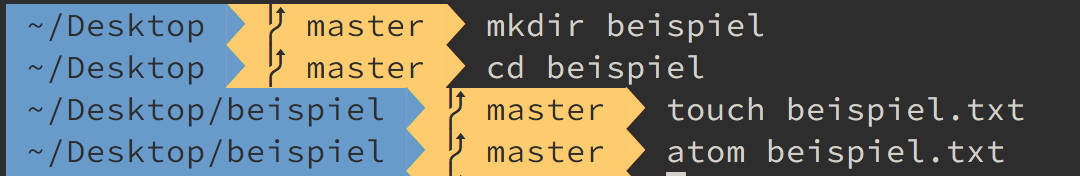
\includegraphics[width=.7\linewidth]{cli-einfaches}
        \caption{Beispiel Terminal}
        \label{fig:sub1}{Hier sehen sie mein Terminal,(
        ich benutze iTerm auf meinem Macbook Pro),
        worin ich gerade
        die Version von meinem Project mithilfe von Git aktualisiere.}
        \end{figure}


        \begin{figure}[ht]
            \centering
            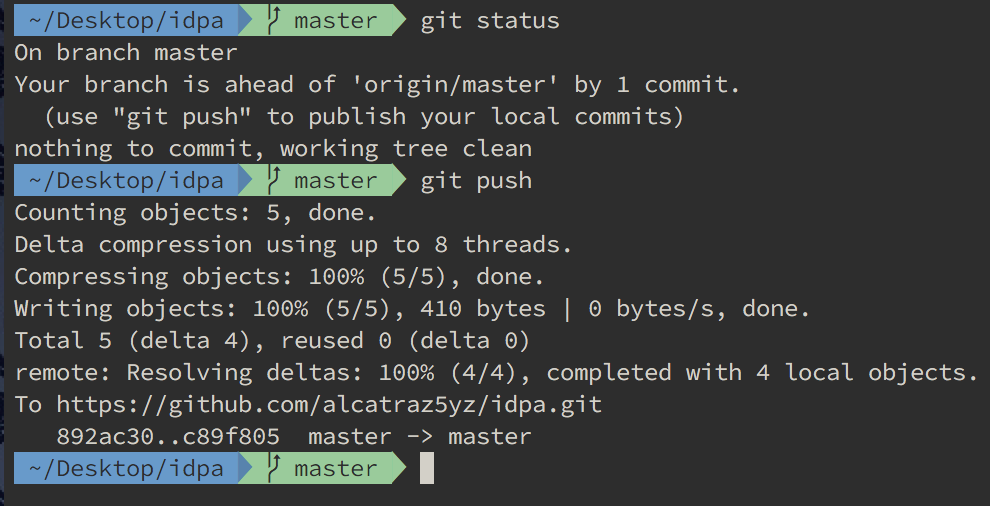
\includegraphics[width=.8\linewidth]{cli-git}
            \caption{Beispiel Termin}
            \label{fig:sub1}{Hier sehen sie mein Terminal,(
            ich benutze iTerm auf meinem Macbook Pro),
            worin ich gerade
            die Version von meinem Project mithilfe von Git aktualisiere.}
            \end{figure}

            \begin{figure}[ht]
                \centering
                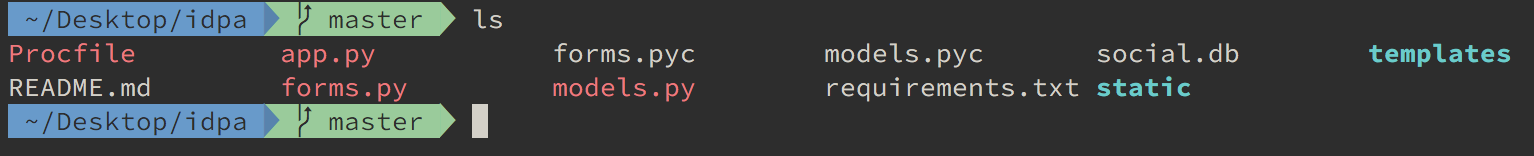
\includegraphics[width=.9\linewidth]{cli-ls}
                \caption{Beispiel Termin}
                \label{fig:sub1}{Hier sehen sie mein Terminal,(
                ich benutze iTerm auf meinem Macbook Pro),
                worin ich gerade
                die Version von meinem Project mithilfe von Git aktualisiere.}
                \end{figure}


            \begin{figure}[ht]
                \centering
                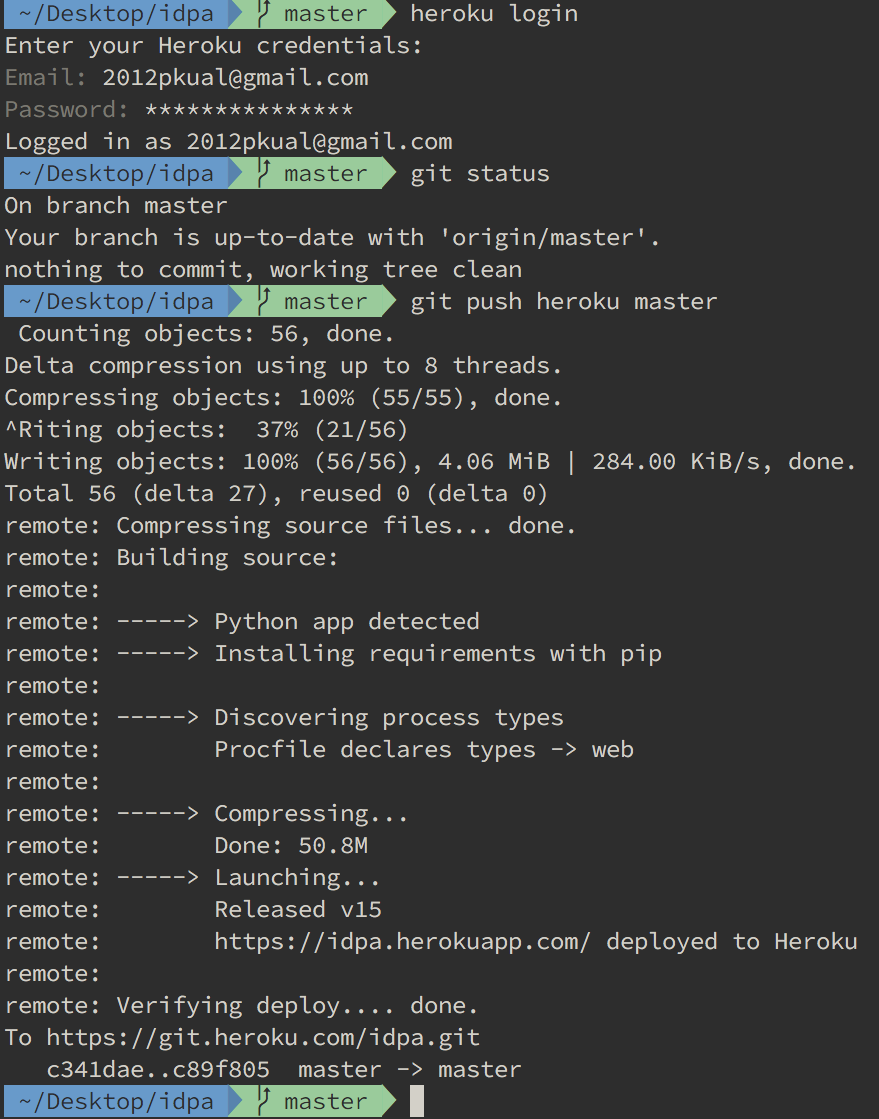
\includegraphics[width=.8\linewidth]{cli-heroku}
                \caption{Beispiel Terminal}
                \label{fig:sub1}{Hier sehen sie mein Terminal,(
                ich benutze iTerm auf meinem Macbook Pro),
                worin ich gerade
                die Version von meinem Project mithilfe von Git aktualisiere.}
                \end{figure}
\cleardoublepage










\section{Erstellen der Seite}
Nun Zeige ich wie ich die Webseite erstellt habe, das heisst ich werde den Code pr?sentieren, und zeigen was er macht.




\section{signup}
\begin{figure}[ht]
    \centering
    
\includegraphics[width=.5\linewidth]{git_logo}
    \caption{Version control}
    \label{fig:sub1}
    \end{figure}

\cleardoublepage













\section{login}
\begin{figure}[ht]
    \centering
    
\includegraphics[width=.5\linewidth]{git_logo}
    \caption{Version control}
    \label{fig:sub1}
    \end{figure}

\cleardoublepage










\section{logout}
\begin{figure}[ht]
    \centering
    
\includegraphics[width=.5\linewidth]{git_logo}
    \caption{Version control}
    \label{fig:sub1}
    \end{figure}

\cleardoublepage























\section{stream}

\begin{figure}[ht]
    \centering
    
\includegraphics[width=.5\linewidth]{git_logo}
    \caption{Version control}
    \label{fig:sub1}
    \end{figure}

\cleardoublepage

\section{paint}


\begin{figure}[ht]
    \centering
    
\includegraphics[width=.5\linewidth]{git_logo}
    \caption{Version control}
    \label{fig:sub1}
    \end{figure}
\cleardoublepage
























\section{Game}
Mein Game werde ich nun gleich pr?sentieren wie die Webseite,das heisst ich werde wieder zeigen was der Code macht und welche bilder usw. er produziert.
\begin{figure}[ht]
    \centering
    
\includegraphics[width=.5\linewidth]{phaser}
    \caption{Version control}
    \label{fig:sub1}
    \end{figure}


    \subsection{Sounds}
    Ich habe 4 verschiedene Arten von Sound ins Game eingebaut.\\
    Ein Sound ist das Ganze Spiel ?ber aktiv und ist sowas wie die Hintergrundmusik des Games.\\
    Der Zweite Sound wird abgespielt wenn entweder das Gameover oder youWin oder Play im Startmenu ausgew?hlt wird.\\
    Der Dritte Sound ist ein Schmerz-Sound der abgespielt wird wenn der Spieler getroffen wird.\\
    Der vierte Sound ist derjenige f?r die Waffe des Spielers, sie wird aktiviert, wenn einer der Meteoriten abgeschossen wird.\\



\subsection{Meine Verwendeten Bilder und Sprites}

\begin{figure}[ht]
\centering
\begin{subfigure}{.5\textwidth}
  \centering
  
\includegraphics[width=.3\linewidth]{diamond}
  \caption{Version control}
  \label{fig:sub1}
\end{subfigure}%
\begin{subfigure}{.5\textwidth}
  \centering
  
\includegraphics[width=.6\linewidth]{dude}
  \caption{phaser}
  \label{fig:sub2}
\end{subfigure}
% \caption{}
% \label{fig:test}
% \caption[short title]{}
\end{figure}


\begin{figure}[ht]
\centering
\begin{subfigure}{.5\textwidth}
  \centering
  
\includegraphics[width=.3\linewidth]{explosion}
  \caption{Version control}
  \label{fig:sub1}
\end{subfigure}%
\begin{subfigure}{.5\textwidth}
  \centering
  \includegraphics[width=.3\linewidth]{titleBG}
  \caption{phaser}
  \label{fig:sub2}
\end{subfigure}
% \caption{}
% \label{fig:test}
% \caption[short title]{}
\end{figure}



\begin{figure}[ht]
\centering
\begin{subfigure}{.5\textwidth}
  \centering
  
\includegraphics[width=.1\linewidth]{ghost}
  \caption{Version control}
  \label{fig:sub1}
\end{subfigure}%
\begin{subfigure}{.5\textwidth}
  \centering
  
\includegraphics[width=.3\linewidth]{loader_bar}
  \caption{phaser}
  \label{fig:sub2}
\end{subfigure}
% \caption{}
% \label{fig:test}
% \caption[short title]{}
\end{figure}




\begin{figure}[ht]
\centering
\begin{subfigure}{.5\textwidth}
  \centering
  
\includegraphics[width=.3\linewidth]{platform}
  \caption{Version control}
  \label{fig:sub1}
\end{subfigure}%
\begin{subfigure}{.5\textwidth}
  \centering
  
\includegraphics[width=.3\linewidth]{sky}
  \caption{phaser}
  \label{fig:sub2}
\end{subfigure}
% \caption{}
% \label{fig:test}
% \caption[short title]{}
\end{figure}




\begin{figure}[ht]
\centering
\begin{subfigure}{.5\textwidth}
  \centering
  \includegraphics[width=.3\linewidth]{spacerock}
  \caption{Version control}
  \label{fig:sub1}
\end{subfigure}%
\begin{subfigure}{.5\textwidth}
  \centering
  \includegraphics[width=.3\linewidth]{star}
  \caption{phaser}
  \label{fig:sub2}
\end{subfigure}
% \caption{}
% \label{fig:test}
% \caption[short title]{}
\end{figure}








\cleardoublepage







\subsection{Game Teil1: index.html}

Im index.html file sind die Referenzen zu den anderen 4
js-files boot/Preloader/StartMenu/Game, als auch der Verweis zum Phaser js-file

\begin{lstlisting}
  <script src="libs/phaser.js"></script>
  <script src="Boot.js"></script>
  <script src="Preloader.js"></script>
  <script src="StartMenu.js"></script>
  <script src="Game.js"></script>
\end{lstlisting}


index.html beinhaltet keine Funktionen welche f?r das Game von Bedeutung w?ren, das heisst der Inhalt des Games wird in den 4 Js-files erstellt.
im index.html file wird nur alles zusammengef?hrt und dann ausgef?hrt weil es ja ein html file ist.
Der Link zum Phaser Hauptfile phaser.js ist auch hier eingebunden.
am Schluss vom FIle wird das File Boot.js aufgerufen



\begin{lstlisting}
    game.state.start('Boot');
\end{lstlisting}



\subsection{Game Teil2: Boot.js}

Im Boot.js werden die Grundlagen f?r das Game erstellt.

\begin{lstlisting}
  create: function() {
        this.input.maxPointers = 1; //nur ein curser
        this.stage.disableVisibilityChange = false; //pauses the game when open another tab
        this.scale.scaleMode = Phaser.ScaleManager.SHOW_ALL;
        this.scale.minWidth = 270;
        this.scale.minHeight = 480;
        this.scale.pageAlignHorizontally = true;//center game
        this.scale.pageAlignVertically = true;//center game
        this.stage.forcePortrait = true;
        this.scale.setScreenSize(true);//force ScreenSize
        this.input.addPointer();
        this.stage.backgroundColor = '#171642';

        this.state.start('Preloader');
    }
\end{lstlisting}

Hier sieht man, dass ich maximal 1 curser habe.\\
Das Game wird gestoppt, wenn ich die Seite verlasse, d.h. ein anderer Tab ?ffne oder das Fenster wechsle.\\
Es wird das Gesamtbild organisiert.\\
Die Hintergrundfarbe des Games ist #171642 was dunkelblau ist.\\
Am Schluss wird das File Preloader.js aufgerufen.\\



\cleardoublepage
\subsection{Game Teil3: Preloader.js}



Mein Game besteht aus 3 Fenstern sozusagen, dem Ladefenster, dem Startmenufenster und dem Game selber.
Hier im Preloader.js wird das Ladefenster kreiert, welches aus Hintergrundbild und Ladebalken besteht.
diese Zwei Bilder wurden im vorherigen File Boot.js geladen.

\begin{lstlisting}
  Survive.Boot.prototype = {
      preload: function() {
          this.load.image('preloaderBar', 'images/loader_bar.png');
      },
\end{lstlisting}

Hier oben wird der Ladebalken geladen

\begin{lstlisting}
  Survive.Boot.prototype = {
  create: function() {
this.stage.backgroundColor = '#171642';
}
}
\end{lstlisting}
Hier oben wird das Hintergrundbild geladen.\\
Im Preloader.js File werden alle Bilder und Sounds welche f?r das Startmenu und das Game sind geladen.


\begin{lstlisting}
          Survive.Preloader.prototype = {
          preload: function () {
          this.load.image('titlescreen', 'images/TitleBG.png');
          this.load.bitmapFont('eightbitwonder', 'fonts/eightbitwonder.png', 'fonts/eightbitwonder.fnt');
          this.load.image('sky', 'images/sky.png');
          this.load.atlasXML('spacerock', 'images/spritesheets/SpaceRock.png', 'images/spritesheets/SpaceRock.xml');
          this.load.image('explosion', 'images/explosion.png');
          this.load.image('platform', 'images/platform.png');
          this.load.image('diamond', 'images/diamond.png');
          this.load.image('star', 'images/star.png');
          this.load.spritesheet('dude', 'images/dude.png', 32, 48);
          this.load.image('ghost', 'images/ghost.png');
          this.load.audio('explosion_audio', 'audio/explosion.mp3');
          this.load.audio('hurt_audio', 'audio/hurt.mp3');
          this.load.audio('select_audio', 'audio/select.mp3');
          this.load.audio('game_audio', 'audio/bgm.mp3');
      },
\end{lstlisting}


Die Animation f?r den Ladebalken:
\begin{lstlisting}
  preload: function () {
        this.preloadBar = this.add.sprite(this.world.centerX, this.world.centerY, 'preloaderBar');
        this.preloadBar.anchor.setTo(0.5, 0.5);
        this.load.setPreloadSprite(this.preloadBar);
        }
\end{lstlisting}

An Schluss wird das File Startmenu.js aufgerufen.\\


\begin{lstlisting}
    game.state.start('StartMenu');
\end{lstlisting}

\cleardoublepage
\subsection{Game Teil4: Startmenu.js}

Im Starmenu erstelle ich das zweite Bild, n?mlich dieses:

\begin{figure}[ht]
    \centering
    \includegraphics[width=.3\linewidth]{foto}
    \caption{}
    \label{fig:sub1}
    \end{figure}

Zuerst kreiere ich das Bild mit dem Text'Press to Start' drauf
\begin{lstlisting}
  image = this.add.image(0, 0, 'titlescreen');
    text = this.add.bitmapText(this.world.centerX-155,
    this.world.centerY+280, 'eightbitwonder', 'Press to Start', 24);
        text.inputEnabled = true;
        text.events.onInputDown.addOnce(this.startGame, this);
\end{lstlisting}

Wenn ich das Bild anklicke, sollte es ja ein ger?usch machen, um mir zu signalisieren, dass es funktioniert hat.
Deshalb baue ich noch das Ger?usch ein.

\begin{lstlisting}
this.audio = this.add.audio('select_audio');
this.audio.play();
\end{lstlisting}
Da ja alles schon geladen ist, muss ich nur es noch einsetzen.\\
Am Schluss wird das File Startmenu.js aufgerufen.\\

\begin{lstlisting}
    game.state.start('Game');
\end{lstlisting}

\cleardoublepage
\subsection{Game Teil5: Game.js}


Am Schluss kreiere ich das dritte Fenster, n?mlich das Game.
Im Game hat es viele Sachen und Aktionen welche kreiert werden m?ssen.








\cleardoublepage






\section{Zusammenfassung}
\cleardoublepage

\section{Summary}
\cleardoublepage




\section{Literaturverzeichnis}
\cleardoublepage




% Appendix starts here
\appendix
\section{Anhang}
Hier sind noch alle Seiten welche ich w?rmstens Empfehle wenn auch du mit
Programmieren starten willst.
idpa.herokuapp.com
meine Webseite auf Github

phaser
flask
texteditors atom/brackets/sublime/
jqueryrain
Css
Git
Github
heroku
teamtreehouse
lynda
codacademy






\end{document}
